\chapter{Konttien orkestrointi\label{orchestration}}

Konttiteknologiaa ja konttien orkestrointia käytetään monilla ohjelmistotuotannon osa-alueilla.
Konttiteknologia mahdollistaa fyysisen palvelimen tai ohjelmistökehittäjän tietokoneen suoritusympäristöstä eroavan vakaan ja toistettavan ympäristön \cite{Watada19}.
Konttiorkestrointialustat hallinnoivat suuria määriä kontteja jaetussa klusterissa mahdollistaen palveluiden replikoinnin, tehokkaan julkaisuketjun, kontitettujen palveluiden monitoroinnin ja virhetiloista toipumisen \cite{Khan17}.

\section{Kontti\label{container}}

Kontti on karsittu ympäristö, joka koostuu palvelusta ja sen tarvitsemista riippuvuuksista.
Kontti tarjoaa vakaan ja suljetun ympäristön palvelun suorittamiselle \cite{Watada19}.
Kontti on riippumaton fyysisestä palvelimesta ja sen ulkopuolisestä ympäristöstä, joka mahdollistaa saman kontin toistamisen muilla palvelimilla ja alustoilla \cite{Saha18}.

Virtuaalikonejulkaisuista poiketen useampi kontti voi jakaa resursseja ja näin ollen esimerkiksi käyttöjärjestelmän ydintä ei tarvitse säilöä erikseen jokaiseen konttiin.
Tämän seurauksena kontit ovat kokonsa ja käynnistysnopeutensa suhteen virtuaalikoneita tehokkaampi ratkaisu \cite{Dua14}.

Yleisesti käytettyjä konttiteknologiapalveluita ovat Docker ja Podman \cite{Abraham20, Bernstein14}.
Docker on suosittu ratkaisu, mutta vaatii toimiakseen aina käynnissä olevan palveluprosessin ja root-oikeudet palvelua suorittavaan käyttöjärjestelmään \cite{Abraham20}.
Nämä tekniset ongelmat ratkaisee esimerkiksi Podman, joka toimii ilman erillistä palveluprosessia ja root-oikeuksia \cite{Gantikow20}.
Konttiteknologiapalveluiden käyttämiä konttien suoritysympäristöjä (\textit{container runtime}) ovat muun muassa containerd ja CRI-O.
Konttien suoristusympäristöjen vaikutus palvelun suorituskykyyn suoraan palvelimelle julkaisemiseen verrattuna on vähäinen \cite{torrez19, espe20}.

\section{Konttiorkestrointialustat\label{platforms}}

Erityisesti mikropalvelupohjaiset järjestelmät saattavat koostua useista sadoista konteista.
Myös saman palvelun replikaatio ja alueellinen hajauttaminen luovat tarpeen hallinnoida suuria määriä kontteja \cite{Khan17}.
Konttiorkestrointialustat ovat järjestelmiä, joiden tehtävä on mahdollistaa suurien konttimäärien hallinnointi.
Konttiorkestrointialustat hallinnoivat konttien resurssien käyttöä, mahdollistavat konttien monitoroinnin ja huolehtivat konttien virhetilanteista toipumisesta \cite{Zhou21}.

Kubernetes on laajalti käytetty konttiorkestrointiratkaisu.
Se on nykyisistä ratkaisuista suorituskyvyltään tehokkain ja myös toiminnallisuuksiltaan kattavin \cite{Jawarneh19}.
Muita ratkaisuja ovat muun muassa \textit{Docker Swarm} ja \textit{Amazon Elastic Container Service} \cite{Khan17}.
Tässä tutkielmassa konttien orkestrointia käsitellään pääasiassa Kuberneteksen kautta.

Kubernetes on alkujaan Googlen kehittämä ja nykyään \textit{Linux Foundation}:in osana toimivan \textit{Cloud Native Foundation}:in hallinnoima avoimen lähdekoodin projekti \cite{Burns22}.
Kubernetes hallinnoi podeiksi kutsuttuja yhdestä tai useammasta kontista koostuvia kokonaisuuksia.
Kubernetes-klusteri muodostuu useista fyysisistä palvelimista tai virtuaalikoneista, joita kutsutaan solmuiksi (\textit{node}) \cite{Medel18}.
Kubernetes mahdollistaa muun muassa seuraavat asiat~\cite{Zhou21}:

\begin{itemize}
\item Resurssien käyttörajojen hallinta (\textit{resource limit control}): Muisti- ja suoritinresurssien minimi- ja maksimimäärän asettamisen konttikohtaisesti.
\item Vuoronvalvonta (\textit{scheduling}): Konttien automaattinen ja optimoitu sijoitus eri solmujen välillä.
\item Kuormituksen tasaaminen (\textit{load balancing}): Kuormituksen jakaminen useiden saman palvelun konttien välillä. 
\item Terveystarkastus (\textit{health check}): Konttien toimivuuden tarkastus ja viallisiin kontteihin reagointi.
\item Vikasietoisuus (\textit{fault tolerance}): Automaattinen uusien konttien luonti ja viallisten tuhoaminen virhetilanteissa.
\item Automaattinen skaalautuminen (\textit{auto-scaling}): Konttien lisääminen tai poistaminen automaattisesti kuormituksen mukaan.
\end{itemize}

Kuva \ref{fig:kubernetes} esittää Kuberneteksen eri komponentit.
Kubernetes-klusteri koostuu useasta podeja suorittavasta solmusta.
Koko klusteria hallinnoi \textit{Control Plane}, joka sisältää klusterin hallinnointiin käytetyn REST-rajapinnan, podien jakautumisesta nodejen välillä huolehtivan vuorontajan sekä pysyväistallennetun avainarvosäilön.
Näiden lisäksi \textit{Control Plane} sisältää useita \textit{Controller manager}-prosesseja, jotka hallinnoivat eri resursseja.
Erityisesti \textit{Cloud controller manager} on komponentti, joka mahdollistaa Kubernetes-klusterin yhdistämisen eri pilvialustojen rajapintojen kanssa \cite{components23}.

\begin{figure}[ht]
\begin{center}
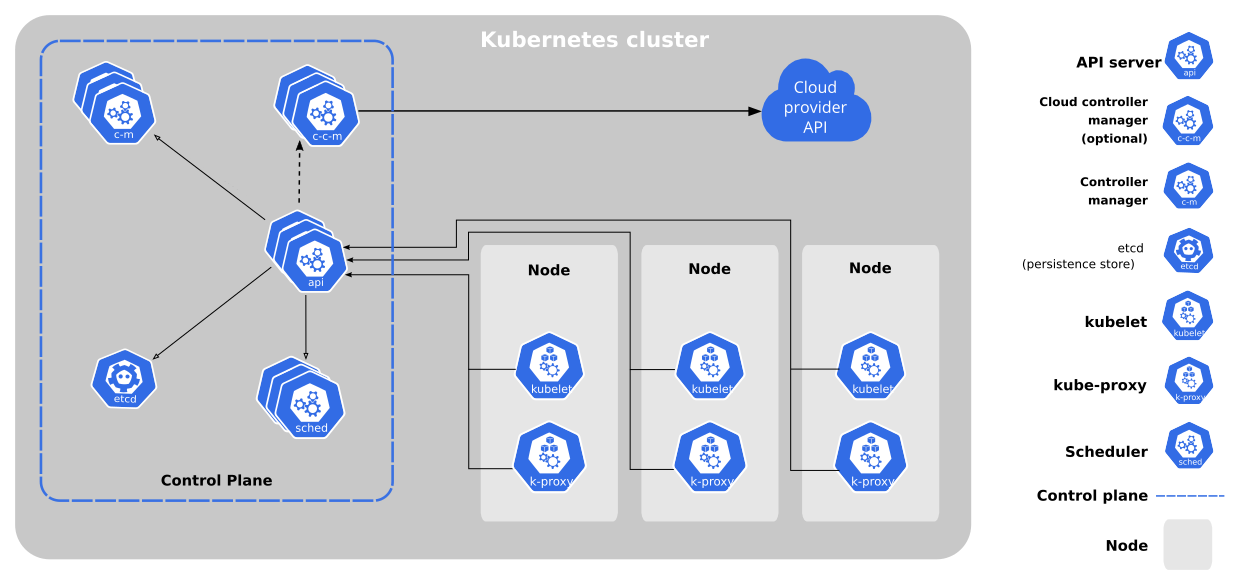
\includegraphics[width=1\textwidth]{figures/kubernetes_components.png}
\caption{Kuberneteksen komponentit \cite{components23}\label{fig:kubernetes}.}
\end{center}
\end{figure}

\section{Konttien orkestrointi DevOps-toimintamallissa\label{orchestration:devops}}

Konttiteknologiaa ja konttien orkestrointia käytetään usein osana DevOps-toimintamalliin perustuvaa ohjelmistotuotantoa \cite{Kang16, Narasimhulu23}.
Konttiteknologian avulla kontitettua palvelua voidaan siirtää eri ympäristöjen, kuten jatkuvan integraation ja toimituksen sekä tuotantoympäristön välillä.
Konttiteknologian avulla koko palvelun ympäristöä voidaan hallita ja riippuvuudet voidaan määritellä konttikohtaisesti.
Tämä konfiguroitavuus johtaa palvelun ennustettavampaan toimintaan ja helpompaan vianmääritykseen \cite{Narasimhulu23}.

Kontin siirrettävyys tukee tehokasta varmennus- ja julkaisuvaihetta DevOps-toimintamal\-lissa, koska samankaltaista konttia voidaan ensin käyttää testauksessa ja sen jälkeen esimerkiksi julkaisualustana toimivalla konttiorkestrointialustalla.
Kontin ympäristön konfiguroitavuus taas auttaa operointi- ja monitorointivaiheissa.
Konfiguroitavuus mahdollistaa koko palvelun ympäristön hallinnan ja riippuvuuksien määrittelyn.
Näin palveluun vaikuttavat ulkoiset tekijät ovat paremmin tiedossa. % cite something?

Kontin erikseen määritettävästä ympäristöstä voi olla hyötyä myös kehitysvaiheessa, koska se mahdollistaa useille kehittäjille samankaltaisen tuotantoympäristöä muistuttavan kehitysympäristön.
Tuotantoympäristöä mahdollisimman paljon muistuttavan kehitysympäristön avulla on mahdollista huomata muuten vasta tuotannossa ilmeneviä ongelmatilanteita jo ennen kuin koodimuutokset on viety tuotantoympäristöön \cite{Narasimhulu23}.
Näin voidaan välttää palvelun toiminnalle aiheutuvia häiriöitä.

Luvussa \ref{platforms} käsitellyt Kuberneteksen tarjoamat konttien orkestrointipalvelut tukevat myös hyvin DevOps-toimintamallia.
Resurssien käytön hallinta, vuoronvalvonta, kuormituksen tasapainottaminen ja automaattinen skaalautuminen ovat kaikki hyödyksi operointivaiheessa.
Terveystarkastus ja vikasietoisuus taas edistävät monitorointivaihetta.
Konttiorkestrointialustan käyttö myös itsessään mahdollistaa konttiteknologian käytön palvelun julkaisuratkaisuna, joka tekee samankaltaisen kontin käytöstä kehityksen, testauksen ja tuotantokäytön aikana mahdollista.

Konttiteknologian ja konttien orkestroinnin käytöstä osana DevOps-toimintamallia on nyt käsitelty paljon etuja.
Konttiteknologian käyttö luo kuitenkin uuden abstraktiokerroksen suoraan palvelimelle julkaisun sijaan, joka voi monimutkaistaa muuten yksinkertaisempaa julkaisuprosessia.
Kontin erillinen ympäristö voi myös johtaa huonompaan ymmärrykseen palvelimen todellisesta ympäristöstä, koska kontin luoma abstraktio piilottaa osaltaan palvelimen toimintaa \cite{Mikkonen22}.

Konttiorkestrointialustan käyttö myös lisää palvelun monimutkaisuutta, varsinkin jos kehittäjillä ei ole aiempaa kokemusta konttien orkestroinnista.
Konttien orkestroinnin tarjoamat edut perustuvat suuren määrän kontteja hallinnointiin automaattisesti \cite{Khan17}.
Näin ollen yksinkertaisen palvelun, kuten muutamasta kontista koostuvan itsenäisen sovelluksen, osalta konttiorkestrointialustan käyttö voi turhaan monimutkaistaa ohjelmistoinfrastruktuuria.
Seuraavaksi tarkastellaan muita julkaisutapoja ja niiden soveltuvuutta DevOps-toimintamallin mukaiseen ohjelmistotuotantoon.
Näitä julkaisutapoja verrataan myös konttiteknologian ja konttien orkestroinnin käyttöön.
